\chapter{Dynamic Author-Topic Model}
\label{chapterlabel3}

\section{Motivation}

The question of "What is this news article about?" is what we want to answer from our proposed model.At the moment the news on BBC websites are tagged which is used to indicate the cluster of the news, for example,Politics\footnote{http://www.bbc.co.uk/news/politics}, Education\footnote{http://www.bbc.co.uk/news/education}, UK\footnote{http://www.bbc.co.uk/news/uk} and Sport\footnote{http://www.bbc.co.uk/sport} etc. However, the granularity or topic here is so coarse that the hidden relations among news and semantic content of a news cannot be specified, and also manual tagging news is so expensive and not practical for a large corporus of news. 

In order to structure the unstructured news better we can use topic models to discover the hidden thematic 
structure of the news and cluster the news collection in a better organization, so that when new data (query or news document) arrives it can be properly fitted into the estimated topic structure. LDA is one possible solution to this problem that models the relation of word-topic, topic-document correctly, which will be beneficial for news classification and clustering. 

However, most of the topic models, such as LDA, and Author Topic model are under the assumption that the documents are exchangeable in the corporus, which means that its probability is invariant to permutation. 

News, is a rolling stream of stories - by definition they live in the present, and evolve over time. So one key challenge we want to solve is, instead discovering static latent topics, we consider news as a continuously streaming of a sequence of documents, its topic distribution change with time with previously salient topics fading-off. For example, on the WAT application of BBC News Lab\footnote{http://wat.bbcnewslabs.co.uk/}, which is a tool to compare coverage on different topics across different media sources using data from the BBC News Labs Juicer, we can obviously see the evolution of "hot topics" on the media.When searching for UK-related news on BBC, obviously we can see the topic distribution of UK news differ from month to month, \textit{murder} appears in May's top topics because of the death of care worker Saima Khan on 23 May in Luton with her sister on \textit{murder} charge. And in June media was focusing on the referendum which is a vote held on Thursday 23 June, to decide whether the UK should leave or remain in the European Union. And British turns to UEFA Euro 2016 in July with D-day approaching and start to welcome the Rio Olympics from middle of July.
\begin{figure}[h]
\centering
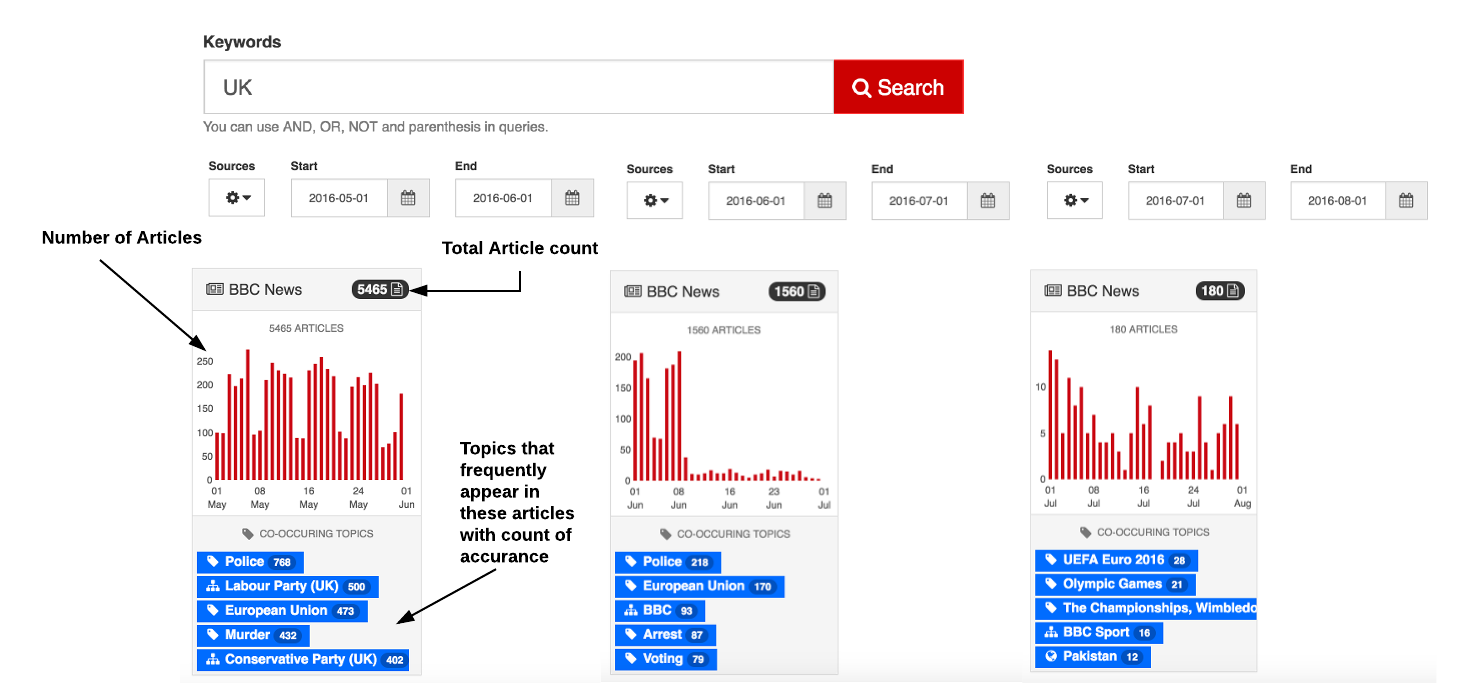
\includegraphics[width=\textwidth]{figures/BBC_wat.png}
\caption{Example of the topic evolution on BBC News: Who's talking about what ?}
\label{fig:bbc_wat}
\end{figure}

The other challenge is to apply author-topic (AT) model for the news collection which simultaneously model the content of the document and also the interest of the authors. The advantage of AT model is that besides representing each news with a mixture of topics, the \textit{author} is also modeled by determining the mixture weights for different topics for a single news, each \textit{author} is associated with a multinomial distribution over topics. This generative model perfectly fits in the corporus of BBC news, since for BBC news there is a virtual \textit{author} for each of the news, which is its category, as shown in ~\ref{tab:news_category}. For news in different categories their prose style will differ in the aspects of vocabulary use,  sentence structure, as well as the way in which stories present the information in terms of relative importance, tone, and intended audience. 

So the BBC news can be assumed to be generated in the following way, as shown in Figure~\ref{fig:author_diagram}.

\begin{enumerate}
   \item For each topic $k \in [1,K]$
   \begin{enumerate}
     \item Draw a multinomial $\vec{\phi_k}$ from a Dirichlet prior $\vec{\beta}$
    \end{enumerate}
   \item For each author $a \in [1,A]$
   \begin{enumerate}
     \item Draw a multinomial $\vec{\theta_a}$ from a Dirichlet prior $\vec{\alpha}$
    \end{enumerate}
    \item For each news $m \in [1,M]$
   \begin{enumerate}
     \item For each word $n \in [1,N_m]$ in document $m$
     \begin{enumerate}
            \item Draw an author $x_{m,n}$ uniformly from the group of authors $a_M$
            \item Draw a topic assignment $z_{m,n}$ from per-author multinomila distribution over topic $\vec{\theta_{x_{m,n}}}$
            \item Draw a word $w_{m,n}$ from multinomial $\vec{\phi_{z_{m,n}}}$
    \end{enumerate}
    \end{enumerate}
        
\end{enumerate}

In the above process the posterior distribution of topics are dependent on the information form the authors as well as the text of the news. The parameterization of the AT model can be seen in Section ~\ref{Author-Topic model}

\begin{figure}[h]
\centering
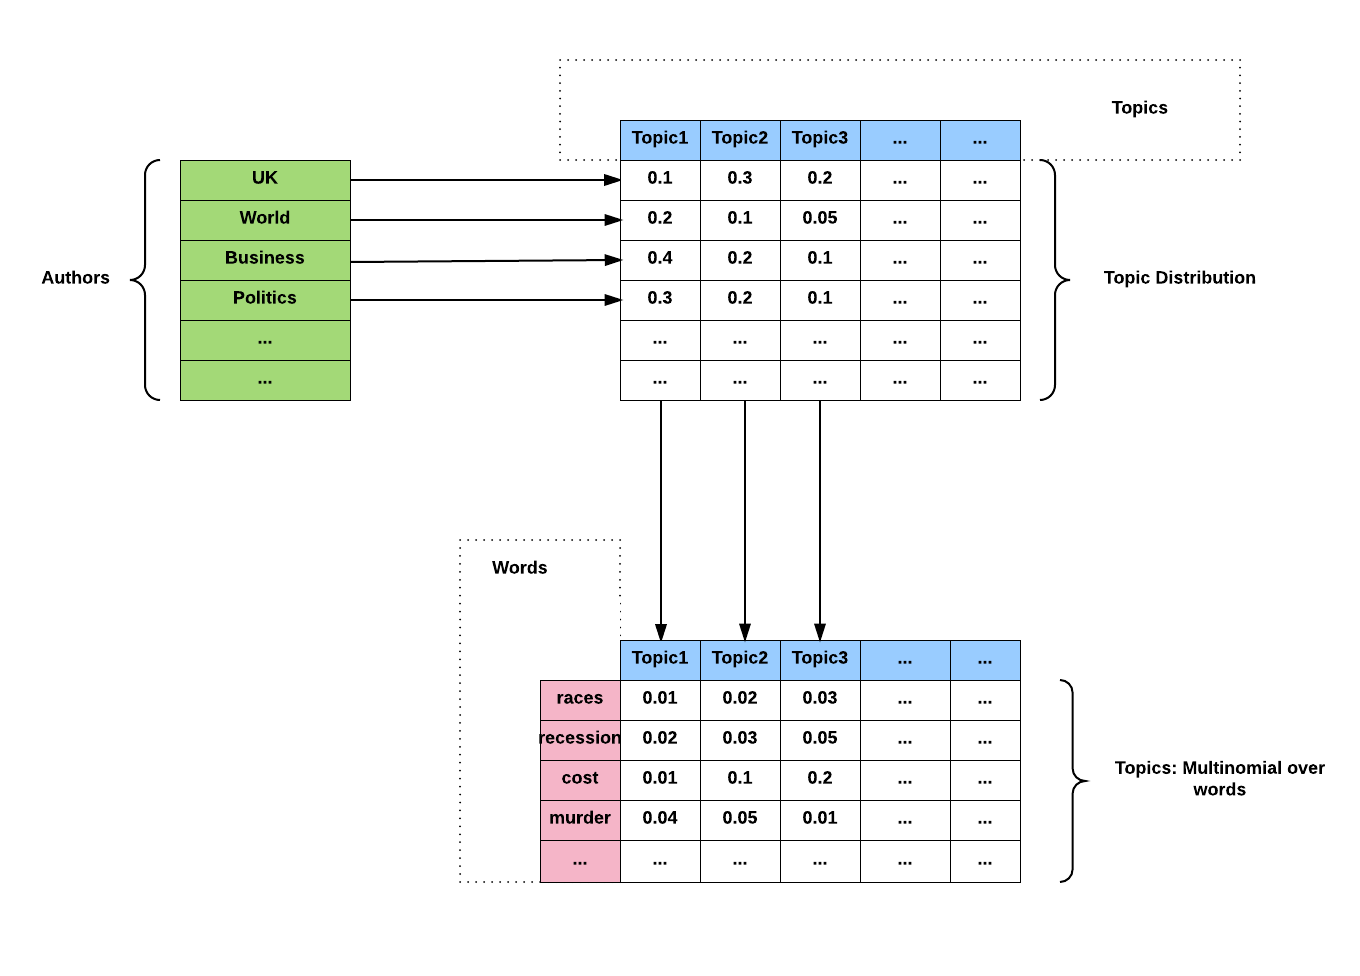
\includegraphics[width=\textwidth]{figures/author_diagram.png}
\caption{Illustration of generative models for BBC news document}
\label{fig:author_diagram}
\end{figure}


Therefore in order to encompass the extra-feature of the news, namely its category, in our model, the AT model is used as the basis of our dynamic model to overcome the above two challenges. Here we define the concepts of \textbf{\textit{topic}} and \textbf{\textit{author}} as follows: 
\begin{itemize}
  \item A \textbf{\textit{topic}} is a subject discussed in one or more news. Examples of topics include events such as "UK referendum" entities such as "David Cameron " and long-standing subjects such as "UK Politics". Each topic is assumed to be represented by a multinomial distribution of words.
  \item An \textbf{\textit{author}} is a category of BBC news which groups topics belonging to a common subject
  area together. Examples of authors include BBC news categories of "UK", "World", "Eduction", "Health", etc, as listed in ~\ref{tab:news_category}
  \end{itemize}
The model we propose here is Dynamic Author-Topic (DAT) model which draws upon the strength of author-topic model and dynamic topic model. Considering the temporal nature of news we assume the topic distributions of news will evolve over time frames (a day, a week or a month), and the inferred topic distribution in the past news documents will become the evidence of those for the current new. In each time frame, we assume the news are generated based on author-topic model. Information about which topics are associated to which author and the representation of the content of each news document in terms of topics are derived and used for the next time frame. The details are discussed in the following sections.

\section{Task Description}\label{taskdescription}
The task that is addressed in this thesis can fall in the following 3 aspects

\begin{itemize}
  \item \textbf{Tagging}: Based on the content and time of the news we are able to automatically tag the news with an author (category)
  \item \textbf{Summarization}: Based on the author-topic distribution we are able to what topics are most discussed in one type of news
  \item \textbf{Dynamics}: We are able to monitor the changes of event of interest for the news over time
\end{itemize}

The input of our model will be the BBC news text in a range of time,

\begin{figure}[h]
\centering
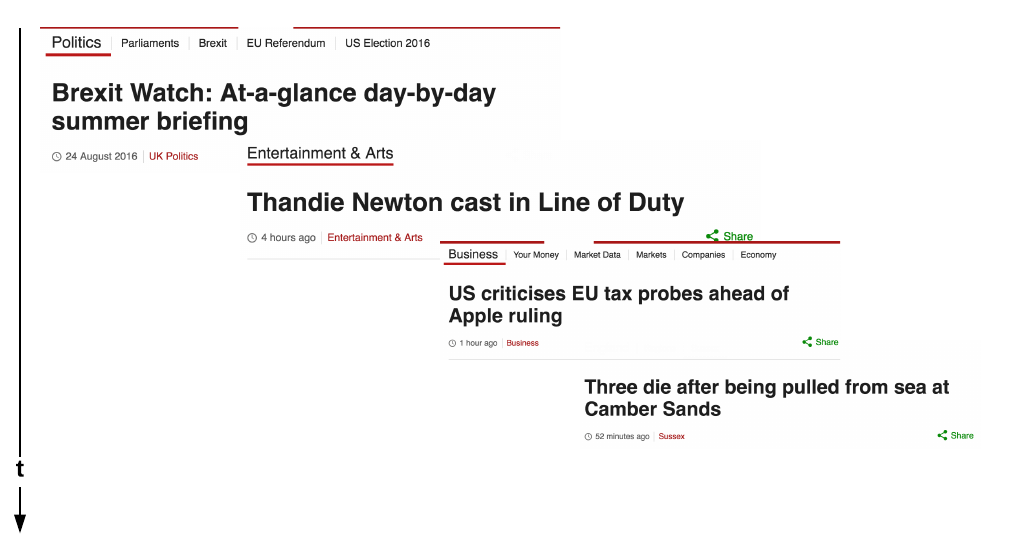
\includegraphics[width=\textwidth]{figures/input.png}
\caption{Input: BBC News over time}
\label{fig:input}
\end{figure}

The output will satisfies the above 3 aspects, as shown in Figure ~\ref{fig:output}
\begin{figure}[h]
\centering
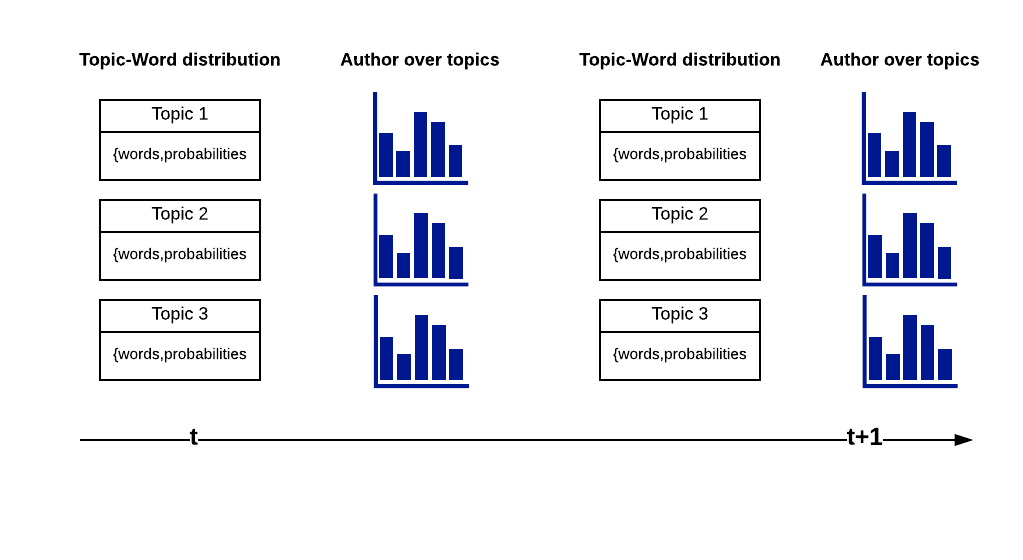
\includegraphics[width=\textwidth]{figures/output.png}
\caption{Output: Temporal evolution of topics and authors’ proportion over the topics }
\label{fig:output}
\end{figure}



Mathematically, the author-topic and topic-words distribution are changing dynamically with news stream in, our dynamic model is essentially a function $f$ that satisfies:
\begin{equation}
\label{eq:task}
\mathbf{m}_{\le t}=\{\ldots, \mathbf{m}_{t-2}', \mathbf{m}_{t-1}', \mathbf{m}_t'\}
\stackrel{f}{\longrightarrow} \boldsymbol W'_{\boldsymbol a,\boldsymbol k}_{\le t}=\{\{\mathbf{w}_1', \mathbf{w}_2', \ldots, \mathbf{w}_K'\},\{\mathbf{w}_1', \mathbf{w}_2', \ldots, \mathbf{w}_A'\}\}
\end{equation}

in which $\mathbf{m}_{\le t}$ represents news stream with $\mathbf{m}_t'$ being the most recent \textit{set} news, arring at time $t$, with our dynamic model it results in  $\boldsymbol W'_{\boldsymbol a,\boldsymbol k}$ is the resulting set of 3-tuple, $\{w,a,k\}$, which represents word $w$ and the author $a$ and topic $k$ assigned to it, with $\mathbf{w}_k'$ being the words set associated with topic $k$,  with $\mathbf{w}_a'$ being the words set associated with author $a$-th.

$\mathbf{m}'_t$ comprises a the stream of news at time $t$, with each news $m$ being represented by a sequence of words appearing in $m$, coming from the vocabulary $\boldsymbol w$. % and $t$ is the creation time of the document $d$.
%$\mathbf{d}'_t$ comprises a set of short text documents, with each document being represented by a tuple $\langle \mathbf{w}_d, t \rangle$ where $\mathbf{w}_d$ is a sequence of words appearing in document $d$, coming from a vocabulary $\mathbf{V}=\{ v_1, v_2, \ldots, v_V\}$, and $t$ is the creation time of the document $d$. 

Based on $\boldsymbol W'_{\boldsymbol a,\boldsymbol k}$ we are able to calculate the author-topic and topic-word distribution to see the topic evolution over time.
Table ~\ref{tab:notation-des} summarises the main notations that we have used in our dynamic author-topic model.
\begin{table}[h]
\center
\vspace{-1pt}
\caption{Notation used in the Dynamic Author-topic model}
\label{tab:notation-des}
\small
\begin{tabular}{ll}
Symbol & Description\\
\hline

$\bs{K}$ & Number of latent topics\\
$\bs{M}$ & Number of news\\
$\bs{A}$ & Number of unique authors\\
$\bs{A_m}$ & Number of authors in document $m$\\
$\bs{V}$ & Number of unique word tokens in the whole news corpus\\
$T$ & Number of time frames  \\
$N_{\text{m}}$ & Number of word tokens in news m\\
$k$ & Topic index,  $k \in [1,\bs{K]$ \\
$m$ & News index,  $m \in [1,M]$ \\
$a$ & Author index,  $a \in [1,\bs{A}]$ \\
$t$ & Time frame index, $t \in [1,T]$\\
$n$ & Word index in document $m$,  $n \in [1,N_{\text{m}}]$ \\
$v$ & Word index in the whole news document corpus,  $v \in [1,V]$ \\
$\boldsymbol a$ & Set of all authors \\
$\boldsymbol k$ & Set of all topics \\
$\boldsymbol m$ & Set of all news \\
$\boldsymbol m'_t$ & Set of news at time t\\
$\boldsymbol w$ & Words set for all news \\
$\boldsymbol w'_{a}$ & Words set comprising words associated with author $a$ \\
$\boldsymbol w'_{k}$ & Words set comprising words associated with topic $k$ \\
$\boldsymbol W'_{\boldsymbol a,\boldsymbol k}$ & The set of 3-tuple, $\{w,a,k\}$, which represents word $w$ and the author $a$ and topic $k$ assigned to it \\
$\boldsymbol w_m$ & Words set for news $m$ \\
$\alpha_{t}$ & Parameter of topic Dirichlet prior to $\theta$ at time $t$ \\
$\beta{t}$ & Parameter of word Dirichlet prior to $\phi$ at time $t$ \\
$a_m$ & Authors in news m,  $a_m \in [1,\bs{A]$ \\
$\theta_{a,t}$ & Dynamic multinomial distribution of topics specified to author $a$ at time $t$ \\
$\phi_{k,t}$ & Dynamic multinomial distribution of words specified to topic $k$ at time $t$ \\
$x_{m,n}$ & Author associated to $w_{m,n}$ \\
$z_{m,n}$ & Topic associated to $w_{m,n}$ \\
$w_{m,n}$ & $n_{th}$ word in doc $n$ \\



\end{tabular}
\end{table}

\section{Dynamic Author-Topic Model}
To meet the requirements discussed in ~\ref{taskdescription}, so that the event interests of the news can be  














The parameterization of the proposed dynamic author-topic model is as follows:
\begin{eqnarray*} \label{eq:dat}
\boldsymbol{\Theta}_{a,t} | \boldsymbol{\alpha_{a,t}}
\boldsymbol{\Theta}_{a,t-1}
& \sim & \text{Dirichlet}{\boldsymbol{\alpha_{a,t}}
\boldsymbol{\Theta}_{a,t-1}}\\
\boldsymbol{\Phi_{k,t}} | \boldsymbol{\beta_{k,t}}\boldsymbol{\Phi_{k,t-1}} & \sim & \text{Dirichlet}(\boldsymbol{\beta_{k,t}}\boldsymbol{\Phi_{k,t-1}})\\
z_{m,n} | \boldsymbol{\Theta_{x_{m,n},t}} & \sim & \text{Multinomial}(\boldsymbol{\Theta_{x_{m,n},t}})\\
w_{m,n} | \boldsymbol{\Phi_{z_{m,n},t}} & \sim & \text{Multinomial}(\boldsymbol{\Phi_{z_{m,n},t}})\\
x_{m,n} | {A_{m}} & \sim & \text{Multinomial}(1/A_m)\\

\end{eqnarray*}

\begin{figure}[h]
\centering
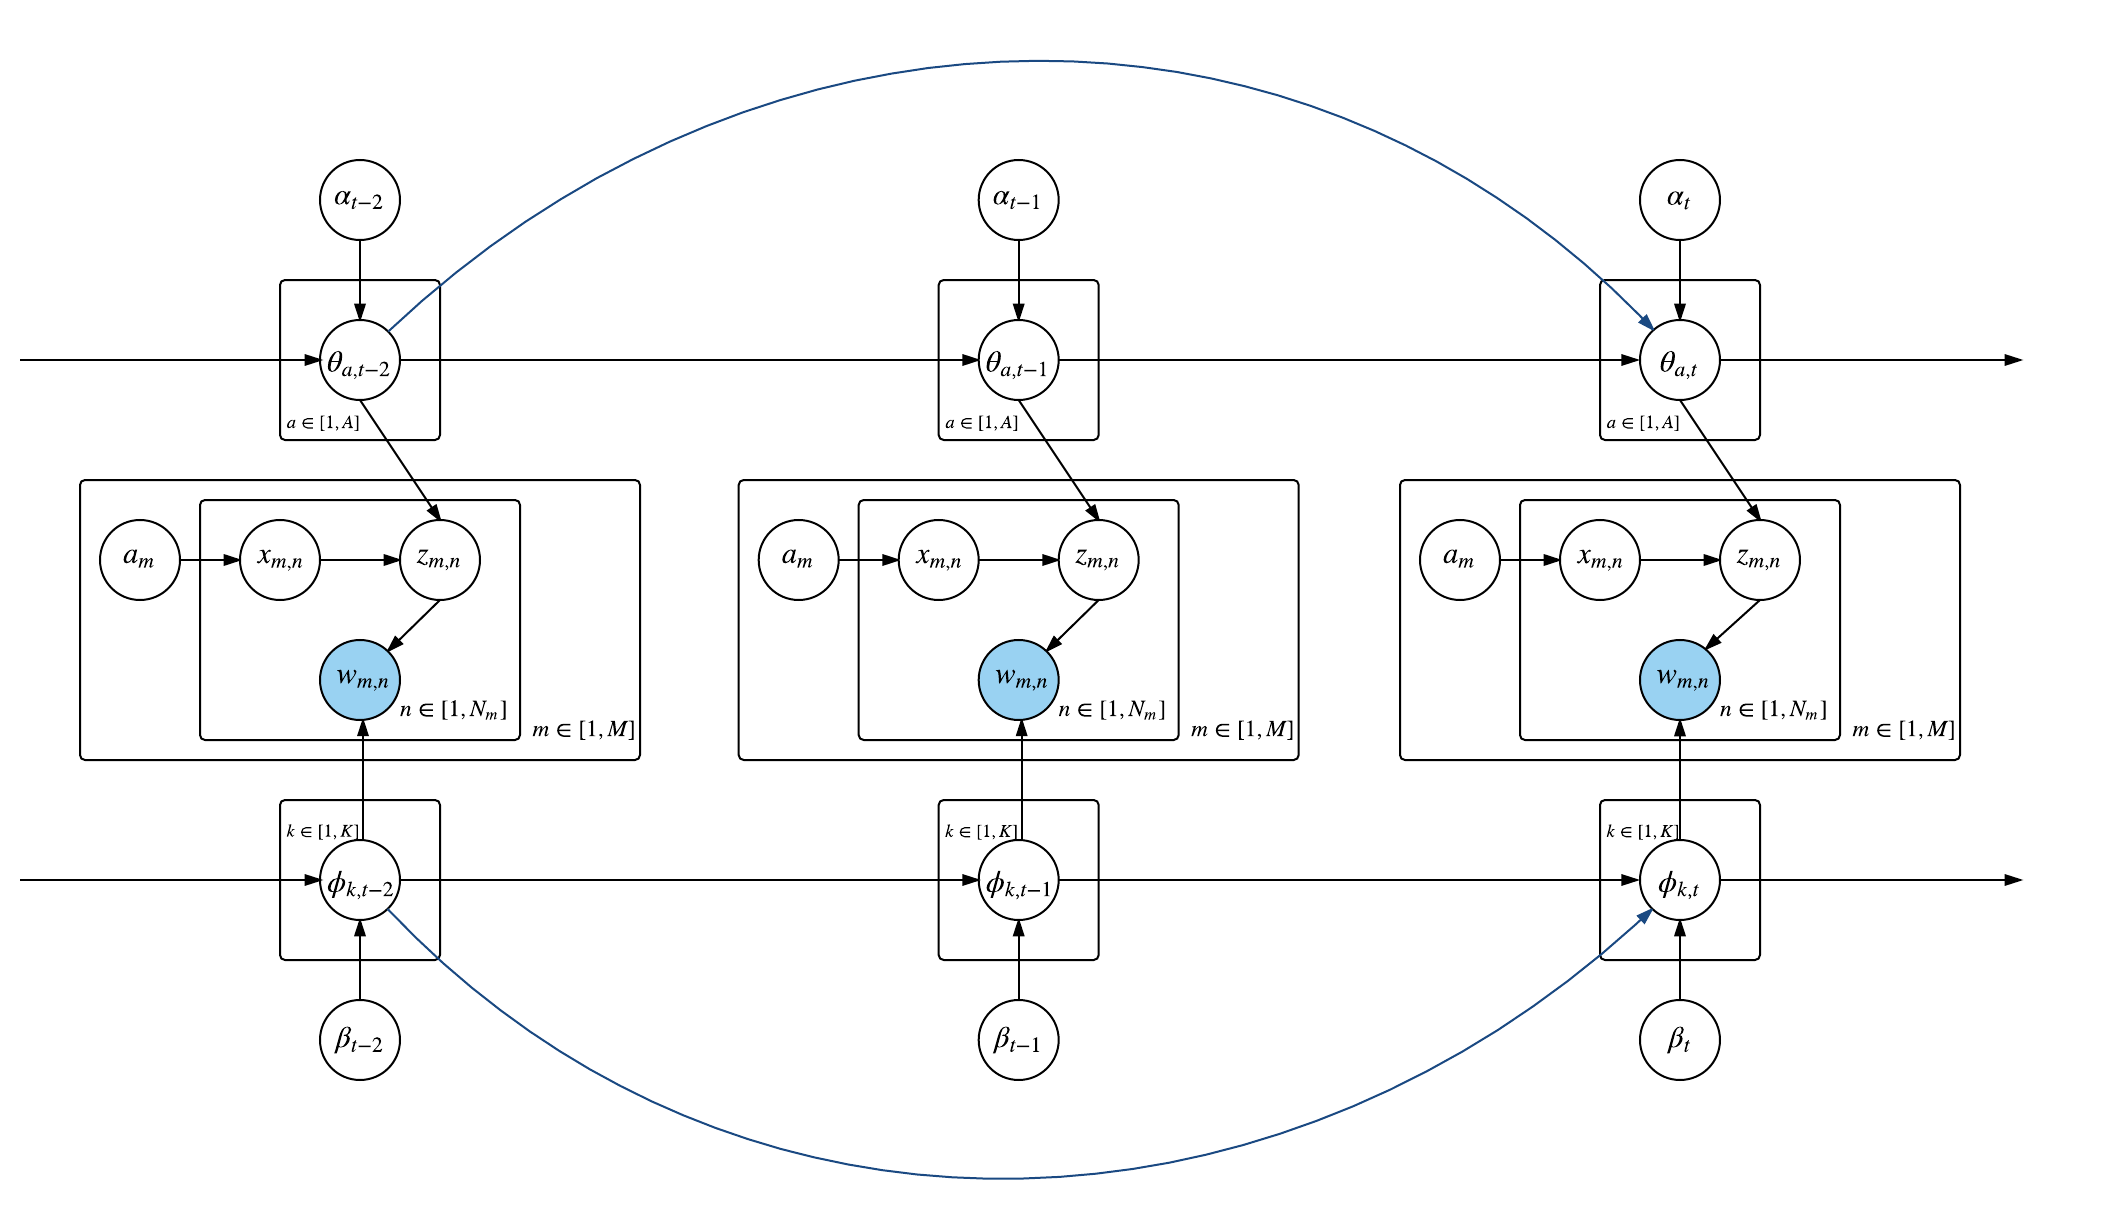
\includegraphics[width=\textwidth]{figures/ATOT_Graphic.png}
\caption{Graphical representation of our dynamic author-topic model, DAT model. Note that short term dependency DAT model excludes the two blue curved lines , the long term dependency DAT model includes the two lines.}
\label{fig:atot}
\end{figure}









\section{Model Inference}

Similar to LDA model, based on the algorithm proposed by \cite{blei2003latent} to calculate the approximate maximum likelihood estimates for $\boldsymbol{\phi}$ as well as the hyperparameter of the prior $\boldsymbol{\theta}$, the Markov Chain Monte Carlo (MCMC) is used for inference, MCMC is an approach to obtain the sample from the complicated probability distributions, to allow a Markov chain to converge to a targeted distribution and the drawing the samples from the Markov chain \cite{gilks1996introducing}. Gibbs Sampling is used here for the inference in which the next state is arrived by sampling all variables from their distribution sequentially when conditioned on the current values of all other variables and the data.
in the above Gibbs sampling procedure, we need to calculate the conditional distribution first, which is
\begin{equation}
P({z}_{m, n, t},{x}_{m, n, t}| \mathbf{w}_t,\mathbf{z}_{\neg(m, n, t)}, \mathbf{x}_{\neg(m, n, t)},\mathbf{a_t},\alpha_t, \beta_t,\boldsymbol{\Phi}_{t-1}, \boldsymbol{\Theta}_{t-1})
\label{eq:conditional}
\end{equation}
where $\mathbf{z}_{\neg(m, n, t)}, \mathbf{x}_{\neg(m, n, t)}$ represents the topic, author assignments for all the word tokens in the news corpus except for $w_{m,n}$. We can begin with the joint distribution,
\begin{equation}
P(\mathbf{w}_t, \mathbf{z}_t ,\mathbf{x}_t| \alpha_t, \beta_t,\mathbf{a}, \boldsymbol{\Phi}_{t-1}, \boldsymbol{\Theta}_{t-1})
\end{equation}
so that we can take advantage of the conjugate priors to simplify the integrals. The symbols used here are all defined in Table~\ref{tab:notation-des}. The whole process of Gibbs sampling derivation for our dynamic author-topic model is listed as follows.
\begin{align*}
\multicolumn{2} =   &  \math{P}({z}_{m, n, t},{x}_{m, n, t}| \mathbf{w}_t,\mathbf{z}_{\neg(m, n, t)}, \mathbf{x}_{\neg(m, n, t)},\mathbf{a_t},\alpha_t, \beta_t,\boldsymbol{\Phi}_{t-1}, \boldsymbol{\Theta}_{t-1})
\displaybreak[3]\\
\propto & \quad P(\mathbf{w}_t, \mathbf{z}_t ,\mathbf{x}_t| \alpha_t, \beta_t,\mathbf{a_t}, \boldsymbol{\Phi}_{t-1}, \boldsymbol{\Theta}_{t-1}) \displaybreak[3]\\
& \hspace{-0.1in}\text{based on the graphical model in Figure ~\ref{fig:atot}, and integrate on $\boldsymbol{\Phi}$ and $\boldsymbol{\Theta}$ it becomes}\displaybreak[3]\\
= & \quad  P(\mathbf{w}_t | \mathbf{z}_t, \mathbf{\beta}_t,\boldsymbol{\Phi}_{t-1})\times P(\mathbf{z}_t | \boldsymbol{\Theta}_{t-1}, \alpha_t, \mathbf{x}_t) \times P(\mathbf{x}_t | \mathbf{a}_t) \displaybreak[3]\\
= & \quad \int P(\mathbf{w}_t | \mathbf{z}_t, \boldsymbol{\Phi}_t) P(\boldsymbol{\Phi}_t | \boldsymbol{\Phi}_{t-1}, \beta_t) d\boldsymbol{\Phi}_t \int P(\mathbf{z}_t | \mathbf{x}_t, \boldsymbol{\Theta}_t) P(\boldsymbol{\Theta}_t | \boldsymbol{\Theta}_{t-1}, \alpha_t) d\boldsymbol{\Theta}_t \displaybreak[3]\\
&  \times P(\mathbf{x}_t | \mathbf{a}_t)\displaybreak[3]\\
& \hspace{-0.1in}\text{we then rewrite the probabilistic distribution from the way of vector to that of scalar, }\\
& \hspace{-0.1in}\text{for example, $P(\mathbf{w}_t | \mathbf{z}_t, \boldsymbol{\Phi}_t)$ can become the the product of $P({w}_{m, n, t} | \phi_{t, z_{m,n}})$      across the}\\
& \hspace{-0.1in}\text{whole corpus, it becomes,}\displaybreak[3]\\
= & \quad \int \prod_{m=1}^{M} \prod_{n=1}^{N_m} P({w}_{m, n, t} | \phi_{t, z_{m,n}}) \prod_{k=1}^K P(\phi_{t, k} | \phi_{t-1,k}, \beta_t) d\Phi_t \displaybreak[3]\\
&  \times \int \prod_{m=1}^{M} \prod_{n=1}^{N_m} P({z}_{m, n, t} | {\theta}_{x_{m,n}},t) \prod_{a=1}^{A}P(\theta_{a,t}|\theta_{a,t-1},\alpha_t) d\Theta_t \displaybreak[3]\\
&  \times \prod_{m=1}^{M} \prod_{n=1}^{N} P({x}_{m, n, t} | {a}_{m,t}) \displaybreak[3]\\
& \hspace{-0.1in}\text{since extract the word $w_{m,n}$ from topic $z_{n,n}$ exactly follow the distribution of $\phi_{z_{m,n}}$, and }\displaybreak[3]\\
& \hspace{-0.1in}\text{also extract topic $z_{m,n}$ from the author $x_{m,n}$ similarly follow the distribution of $\theta_{x_{m,n}}$, so, }\displaybreak[3]\\
= & \quad \int \prod_{k=1}^K \prod_{v=1}^V \phi_{t, v, k}^{n_{(t, v,k)}} \prod_{k=1}^K P(\phi_{t, k} | \phi_{t-1, k}, \beta_t) d\Phi_t \displaybreak[3]\\
&  \times \int \prod_{a=1}^A \prod_{k=1}^K \theta_{t, a, k}^{n_{(t, a,k)}} \prod_{a=1}^A P(\theta_{a,t}|\theta_{a,t-1},\alpha_t) d\Theta_t \times \left(\frac{1}{\prod_{m=1}^M A_m^{N_m}} \right) \displaybreak[3]\\
%
& \hspace{-0.1in}\text{based on the posterior of  Dirichlet distribution \cite{ferguson1973bayesian} }\displaybreak[3]\\
= & \quad \int \prod_{k=1}^K \prod_{v=1}^V \phi_{t,v,k}^{n_{(t,v,k)}} \prod_{k=1}^K \left( \frac{\mathrm{\Gamma} (\sum_{v=1}^V \beta_{(t, k, v)} {\phi_{t-1}})}{\prod_{v=1}^V \mathrm{\Gamma}(\beta_{(t, k, v)} {\phi_{t-1}})} \prod_{v=1}^V \phi_{t, k, v}^{\left(\beta_{(t, k, v)} {\phi_{t-1}} \right) -1} \right) d\Phi_t \displaybreak[3]\\
%
&  \times \int \prod_{a=1}^A \prod_{k=1}^K \theta_{t, a, k}^{n_{(t, a,k)}} \prod_{a=1}^A \left( \frac{\mathrm{\Gamma}(\sum_{k=1}^k \alpha_{(t, k)} \theta_{t-1, k})}{\prod_{k=1}^K \mathrm{\Gamma} (\alpha_{(t, k)} \theta_{t-1, k})} \prod_{k=1}^K \Theta_{t, k}^{\left(\alpha_{(t, k)} {\Theta_{t-1,k}} \right) -1}  \right)  d\Theta_t \displaybreak[3]\\
%
&  \times \left(\frac{1}{\prod_{m=1}^M A_m^{N_m}} \right) \displaybreak[3]\\
%
%
%= & \prod_{z=1}^Z \frac{\mathrm{\Gamma} (\sum_{v=1}^V \beta_{t, z, v} \abbrev{\phi})}{\prod_{v=1}^V \mathrm{\Gamma}(\beta_{t, z, v} \abbrev{\phi})} \int \prod_{z=1}^Z \prod_{v=1}^V \phi_{t, z, v}^{n_{t, z, v}} \prod_{z=1}^Z \prod_{v=1}^V \phi_{t, z, v}^{\beta_{t, z, v} \abbrev{\phi} -1} d\Phi_t \displaybreak[3]\\
%& \times \frac{\mathrm{\Gamma}(\sum_{z=1}^Z \alpha_{t, z} \theta_{t-1, z})}{\prod_{z=1}^Z \mathrm{\Gamma} (\alpha_{t, z} \theta_{t-1, z})} \int \prod_{z=1}^Z \theta_{t, z}^{m_{t, z}}  \prod_{z=1}^Z \theta_{t, z}^{\alpha_{t, z} \theta_{t-1, z} -1} d\Theta_t \displaybreak[3]\\
%
& \hspace{-0.1in}\text{since for different topics , based on d-separation \cite{geiger2013d} their topic-word distribution  }\displaybreak[3]\\
& \hspace{-0.1in}\text{can be regarded as independent from each other, which is the same for author-topic   }\displaybreak[3]\\
& \hspace{-0.1in}\text{distributions, so that the integration of products can be rewritten as product of integrations,}\displaybreak[3]\\
= & \quad \prod_{k=1}^K \frac{\mathrm{\Gamma} (\sum_{v=1}^V \beta_{(t, k, v)} {\phi_{t-1}})}{\prod_{v=1}^V \mathrm{\Gamma}(\beta_{(t, k, v)} {\phi_{t-1}})} \prod_{k=1}^K \int \prod_{v=1}^V \phi_{t, v,k}^{n_{t, v,k}+\beta_{t, k,v} {\phi_{t-1}} -1} d\Phi_t \displaybreak[3]\\
& \times \prod_{a=1}^A \frac{\mathrm{\Gamma}(\sum_{k=1}^K \alpha_{(t, k)} \theta_{t-1, k})}{\prod_{k=1}^K \mathrm{\Gamma} (\alpha_{(t, k)} \theta_{(t-1, k)})} \prod_{a=1}^A \int \prod_{k=1}^K \theta_{t, k}^{n_{t,a,k}+\alpha_{t, k} \theta_{t-1, k} -1} d\Theta_t \displaybreak[3]\\
& \times \left(\frac{1}{\prod_{m=1}^M A_m^{N_m}} \right) \displaybreak[3]\\
& \hspace{-0.1in}\text{according to Euler integral \cite{jeffrey2008handbook},}\displaybreak[3]\\
= & \quad \prod_{k=1}^K \frac{\mathrm{\Gamma} (\sum_{v=1}^V \beta_{t, k, v} {\phi_{t-1}})}{\prod_{v=1}^V \mathrm{\Gamma}(\beta_{t, k, v} {\phi_{t-1}})} \prod_{k=1}^K \frac{\prod_{v=1}^V \mathrm{\Gamma} (n_{t,v,k} + \beta_{t, k, v} {\phi_{t-1}})}{\mathrm{\Gamma} (\sum_{v=1}^V n_{t,v,k} + \beta_{t, k, v} {\phi_{t-1}})} \displaybreak[3]\\
&  \times \prod_{a=1}^A \frac{\mathrm{\Gamma}(\sum_{k=1}^K \alpha_{t, k} \theta_{t-1, k})}{\prod_{k=1}^K \mathrm{\Gamma} (\alpha_{t, k} \theta_{t-1, k})}  \prod_{a=1}^A \frac{\prod_{k=1}^K \mathrm{\Gamma} (n_{t,a,k} + \alpha_{t, k} \theta_{t-1, k})}{\mathrm{\Gamma} (\sum_{k=1}^K n_{t,a, k} + \alpha_{t, k} \theta_{t-1, k})} \displaybreak[3]\\
& \times   \left(\frac{1}{\prod_{m=1}^M A_m^{N_m}} \right) \displaybreak[3]\\
%
\end{align*}
where $n_{t,a,k} = n_{a,t}^(k) $ representing the number of times the author $a$ is assigned to topic $k$, at time $t$, and $n_{t,v,k}$ representing the number of times word token $v$ is assigned to topic $k$, at time $t$.
Applying the chain rule, we can obtain the conditional probability,

\begin{align*}
\multicolumn{2} =   &  \math{P}({z}_{m, n, t},{x}_{m, n, t}| \mathbf{w}_t,\mathbf{z}_{\neg(m, n, t)}, \mathbf{x}_{\neg(m, n, t)},\mathbf{a_t},\alpha_t, \beta_t,\boldsymbol{\Phi}_{t-1}, \boldsymbol{\Theta}_{t-1})
\displaybreak[3]\\
= & \quad \frac{\math{P}({w}_{m, n,t},{z}_{m, n, t},{x}_{m, n, t}| \mathbf{w}_{\neg(m, n, t)},\mathbf{z}_{\neg(m, n, t)}, \mathbf{x}_{\neg(m, n, t)},\mathbf{a_t},\alpha_t, \beta_t,\boldsymbol{\Phi}_{t-1}, \boldsymbol{\Theta}_{t-1})}{\math{P}({w}_{m, n, t}| \mathbf{w}_{\neg(m, n, t)},\mathbf{z}_{\neg(m, n, t)}, \mathbf{x}_{\neg(m, n, t)},\mathbf{a_t},\alpha_t, \beta_t,\boldsymbol{\Phi}_{t-1}, \boldsymbol{\Theta}_{t-1})}
\displaybreak[3]\\
= & \quad \frac{P(\mathbf{w}_t, \mathbf{z}_t,\mathbf{x}_t |  \alpha_t, \beta_t, \boldsymbol{\Phi}_{t-1}, \boldsymbol{\Theta}_{t-1})}{P(\mathbf{w}_{t}, \mathbf{z}_{t,\neg(m,n)},\mathbf{x}_{t,\neg(m,n)} | \alpha_t, \beta_t,a, \boldsymbol{\Phi}_{t-1}, \boldsymbol{\Theta}_{t})} \displaybreak[3]\\
%
= & \quad \frac{P(\mathbf{w}_t, \mathbf{z}_t,\mathbf{x}_t |  \alpha_t, \beta_t, \boldsymbol{\Phi}_{t-1}, \boldsymbol{\Theta}_{t-1})}{P(\mathbf{w}_{t,\neg(m,n)}, \mathbf{z}_{t,\neg(m,n)},\mathbf{x}_{t,\neg(m,n)} | \alpha_t, \beta_t,a, \boldsymbol{\Phi}_{t-1}, \boldsymbol{\Theta}_{t})P(w_{m,n,t} |  \alpha_t, \beta_t, \boldsymbol{\Phi}_{t-1}, \boldsymbol{\Theta}_{t-1})} \displaybreak[3]\\
\propto & \quad \frac{P(\mathbf{w}_t, \mathbf{z}_t,\mathbf{x}_t |  \alpha_t, \beta_t, \boldsymbol{\Phi}_{t-1}, \boldsymbol{\Theta}_{t-1})}{P(\mathbf{w}_{t,\neg(m,n)}, \mathbf{z}_{t,\neg(m,n)},\mathbf{x}_{t,\neg(m,n)} | \alpha_t, \beta_t,a, \boldsymbol{\Phi}_{t-1}, \boldsymbol{\Theta}_{t})} \displaybreak[3]\\
\propto & \quad \prod_{k=1}^K \frac{\mathrm{\Gamma} (\sum_{v=1}^V \beta_{t, k, v} {\phi_{t-1}})}{\prod_{v=1}^V \mathrm{\Gamma}(\beta_{t, k, v} {\phi_{t-1}})} \prod_{k=1}^K \frac{\prod_{v=1}^V \mathrm{\Gamma} (n_{t,v,k} + \beta_{t, k, v} {\phi_{t-1}})}{\mathrm{\Gamma} (\sum_{v=1}^V n_{t,v,k} + \beta_{t, k, v} {\phi_{t-1}})} \displaybreak[3]\\
&  \times \prod_{a=1}^A \frac{\mathrm{\Gamma}(\sum_{k=1}^K \alpha_{t, k} \theta_{t-1, k})}{\prod_{k=1}^K \mathrm{\Gamma} (\alpha_{t, k} \theta_{t-1, k})}  \prod_{a=1}^A \frac{\prod_{k=1}^K \mathrm{\Gamma} (n_{t,a,k} + \alpha_{t, k} \theta_{t-1, k})}{\mathrm{\Gamma} (\sum_{k=1}^K n_{t,a, k} + \alpha_{t, k} \theta_{t-1, k})} \displaybreak[3]\\
& \hspace{-0.1in}\text{applying $\mathrm{\Gamma}(x)=(x-1)\mathrm{\Gamma}(x-1)$ and $\mathrm{\Gamma}(x+m)=\prod_{i=1}^m (x+i-1)\mathrm{\Gamma}(x)$, and considering } \displaybreak[3]\\
& \hspace{-0.1in}\text{that author $a$ is associated with its own topic $z$, the above becomes} \displaybreak[3]\\
\propto & \quad  \left(\frac{n_{t,v,k}+\beta_{t,k,v}\phi_{t-1}-1}{\sum_{v=1}^V \left(n_{t,v,k}+\beta_{t,v,k}\phi_{t-1} \right)-1 } \right) \times   \left(\frac{n_{t,a,k}+\alpha_{t,k} \Theta_{t-1}-1}{\sum_{k=1}^K \left(n_{t,a,k}+\alpha_{t,k}\theta_{t-1} \right)-1 } \right)
\displaybreak[3]\\
\end{align*}

If we manipulate the above formula to turn the above update equations for the topic and author of each token into separated updated ones, which can obtain the following update rules which are suitable for random or systematic scan updates, 
\begin{itemize}
  \item For the topic:
  \begin{align*}
\multicolumn{2} =   &  \math{P}({z}_{m, n, t}| \mathbf{w}_t,\mathbf{z}_{\neg(m, n, t)},\mathbf{x}_t, \mathbf{a_t},\alpha_t, \beta_t,\boldsymbol{\Phi}_{t-1}, \boldsymbol{\Theta}_{t-1})
\displaybreak[3]\\
= & \quad \frac{\math{P}({w}_{m, n, t},{z}_{m, n, t}| \mathbf{w}_{\neg(m, n, t)},\mathbf{z}_{\neg(m, n, t)},\mathbf{x}_t, \mathbf{a_t},\alpha_t, \beta_t,\boldsymbol{\Phi}_{t-1}, \boldsymbol{\Theta}_{t-1})}{\math{P}({w}_{m, n, t}| \mathbf{w}_{\neg(m, n, t)},\mathbf{z}_{\neg(m, n, t)},\mathbf{x}_t, \mathbf{a_t},\alpha_t, \beta_t,\boldsymbol{\Phi}_{t-1}, \boldsymbol{\Theta}_{t-1})}
\displaybreak[3]\\
= & \quad \frac{P(\mathbf{w}_t, \mathbf{z}_t | \mathbf{x}_t, \alpha_t, \beta_t, \boldsymbol{\Phi}_{t-1}, \boldsymbol{\Theta}_{t-1})}{P(\mathbf{w}_{t}, \mathbf{z}_{t,\neg(m,n)} |\mathbf{x}_t, \alpha_t, \beta_t,\mathbf{a_t}, \boldsymbol{\Phi}_{t-1}, \boldsymbol{\Theta}_{t})} \displaybreak[3]\\
= & \quad \frac{P(\mathbf{w}_t, \mathbf{z}_t | \mathbf{x}_t, \alpha_t, \beta_t, \boldsymbol{\Phi}_{t-1}, \boldsymbol{\Theta}_{t-1})}{P(\mathbf{w}_{t,\neg(m,n)}, \mathbf{z}_{t,\neg(m,n)} | \mathbf{x}_{t},\alpha_t, \beta_t,\mathbf{a_t}, \boldsymbol{\Phi}_{t-1}, \boldsymbol{\Theta}_{t})P(w_{m,n} | \mathbf{x}_{t}, \alpha_t, \beta_t, \boldsymbol{\Phi}_{t-1}, \boldsymbol{\Theta}_{t-1})} \displaybreak[3]\\
\propto & \quad \frac{P(\mathbf{w}_t, \mathbf{z}_t | \mathbf{x}_t, \alpha_t, \beta_t, \boldsymbol{\Phi}_{t-1}, \boldsymbol{\Theta}_{t-1})}{P(\mathbf{w}_{t,\neg(m,n)}, \mathbf{z}_{t,\neg(m,n)} | \mathbf{x}_{t},\alpha_t, \beta_t,\mathbf{a_t}, \boldsymbol{\Phi}_{t-1}, \boldsymbol{\Theta}_{t})} \displaybreak[3]\\
%
\propto & \quad \prod_{k=1}^K \frac{\mathrm{\Gamma} (\sum_{v=1}^V \beta_{t, k, v} {\phi_{t-1}})}{\prod_{v=1}^V \mathrm{\Gamma}(\beta_{t, k, v} {\phi_{t-1}})} \prod_{k=1}^K \frac{\prod_{v=1}^V \mathrm{\Gamma} (n_{t,v,k} + \beta_{t, k, v} {\phi_{t-1}})}{\mathrm{\Gamma} (\sum_{v=1}^V n_{t,v,k} + \beta_{t, k, v} {\phi_{t-1}})} \displaybreak[3]\\
&  \times \prod_{a=1}^A \frac{\mathrm{\Gamma}(\sum_{k=1}^K \alpha_{t, k} \theta_{t-1, k})}{\prod_{k=1}^K \mathrm{\Gamma} (\alpha_{t, k} \theta_{t-1, k})}  \prod_{a=1}^A \frac{\prod_{k=1}^K \mathrm{\Gamma} (n_{t,a,k} + \alpha_{t, k} \theta_{t-1, k})}{\mathrm{\Gamma} (\sum_{k=1}^K n_{t,a, k} + \alpha_{t, k} \theta_{t-1, k})} \displaybreak[3]\\
\propto & \quad  \left(\frac{n_{t,v,k}+\beta_{t,k,v}\phi_{t-1}-1}{\sum_{v=1}^V \left(n_{t,v,k}+\beta_{t,v,k}\phi_{t-1} \right)-1 } \right) \times   \left(\frac{n_{t,a,k}+\alpha_{t,k} \Theta_{t-1}-1}{\sum_{k=1}^K \left(n_{t,a,k}+\alpha_{t,k}\theta_{t-1} \right)-1 } \right)
\displaybreak[3]\\
\end{align*}
  \item For the author:
\begin{align*}
\multicolumn{2} =   &  \math{P}({x}_{m, n, t}| \mathbf{z}_t,\mathbf{x}_{\neg(m, n, t)}, \mathbf{a_t},\alpha_t,  \boldsymbol{\Theta}_{t-1})
\displaybreak[3]\\
= & \quad \frac{\math{P}({x}_{m, n, t},{z}_{m, n, t}| \mathbf{x}_{\neg(m, n, t)},\mathbf{z}_{\neg(m, n, t)}, \mathbf{a_t},\alpha_t, , \boldsymbol{\Theta}_{t-1})}{\math{P}({z}_{m, n, t}| \mathbf{x}_{\neg(m, n, t)},\mathbf{z}_{\neg(m, n, t)}, \mathbf{a_t},\alpha_t,  \boldsymbol{\Theta}_{t-1})}
\displaybreak[3]\\
= & \quad \frac{P(\mathbf{x}_t, \mathbf{z}_t | \mathbf{a_t}, \alpha_t, \boldsymbol{\Theta}_{t-1})}{P(\mathbf{z}_{t}, \mathbf{x}_{t,\neg(m,n)} | \mathbf{a_t},\alpha_t,  \boldsymbol{\Theta}_{t})} \displaybreak[3]\\
= & \quad \frac{P(\mathbf{x}_t, \mathbf{z}_t | \mathbf{a_t}, \alpha_t, \boldsymbol{\Theta}_{t-1})}{P(\mathbf{x}_{t,\neg(m,n)}, \mathbf{z}_{t,\neg(m,n)} | \alpha_t, \mathbf{a_t},  \boldsymbol{\Theta}_{t})P(z_{m,n} |  \alpha_t, \boldsymbol{\Theta}_{t-1})} \displaybreak[3]\\
\propto & \quad \frac{P(\mathbf{x}_t, \mathbf{z}_t |  \alpha_t, \mathbf{a_t}, \boldsymbol{\Theta}_{t-1})}{P(\mathbf{x}_{t,\neg(m,n)}, \mathbf{z}_{t,\neg(m,n)} | \alpha_t, \mathbf{a_t},  \boldsymbol{\Theta}_{t})} \displaybreak[3]\\
%
\propto & \quad  \prod_{a=1}^A \frac{\mathrm{\Gamma}(\sum_{k=1}^K \alpha_{t, k} \theta_{t-1, k})}{\prod_{k=1}^K \mathrm{\Gamma} (\alpha_{t, k} \theta_{t-1, k})}  \prod_{a=1}^A \frac{\prod_{k=1}^K \mathrm{\Gamma} (n_{t,a,k} + \alpha_{t, k} \theta_{t-1, k})}{\mathrm{\Gamma} (\sum_{k=1}^K n_{t,a, k} + \alpha_{t, k} \theta_{t-1, k})} \displaybreak[3]\\
\propto & \quad   \left(\frac{n_{t,a,k}+\alpha_{t,k} \Theta_{t-1}-1}{\sum_{k=1}^K \left(n_{t,a,k}+\alpha_{t,k}\theta_{t-1} \right)-1 } \right)
\displaybreak[3]\\
\end{align*}
  
\end{itemize}

Based on the above inference, the multinomila parameter sets $\Theta$ and $\Phi$ can be obtained, according to the definitions as multinomial distributions with Dirichlet prior, to apply the Bayes' rule we will get,
\begin{align*} \label{theta}
P(\boldsymbol{\Theta_{a,t}}|\mathbf{z_t},\mathbf{x_t},\mathbf{\alpha_t},\boldsymbol{\Theta_{a,t-1}}) & = \frac{P(\boldsymbol{\Theta_{a,t}},\mathbf{z_t}|\mathbf{x_t},\mathbf{\alpha_t},\boldsymbol{\Theta_{a,t-1}})}{P(\mathbf{z_t}|\mathbf{x_t},\mathbf{\alpha_t},\boldsymbol{\Theta_{a,t-1}})} \\
 & = {\frac{1}{Z_\boldsymbol{\Theta_{a,t}}}}\prod_{(m,n):x_{m,n}=a}P(z_{m,n}|\boldsymbol{\Theta}_{a,t})P(\boldsymbol{\Theta}_{a,t}|\alpha_t,\boldsymbol{\Theta}_{a,t-1})\displaybreak[3]\\
 & = {\frac{1}{Z_\boldsymbol{\Theta_{a,t}}}}\prod_{k=1}^{K}\theta_{a,k}^{n_{a,k}} \times \frac{\mathrm{\Gamma}(\sum_{k=1}^K \alpha_{t, k} \theta_{t-1, k})}{\prod_{k=1}^K \mathrm{\Gamma} (\alpha_{t, k} \theta_{t-1, k})} \prod_{k=1}^{K}\theta_{a,k}^{\alpha_{t,k}\theta{(t-1),k,a}-1}\\
 & = {\frac{1}{Z_\boldsymbol{\Theta_{a,t}}}}\prod_{k=1}^{K}\theta_{a,k}^{n_{a,k}+\alpha_{t,k}\theta{(t-1),k,a}-1}\\
& = \text{Dirichelet}{(\boldsymbol{\Theta}_{a,t}|\boldsymbol{n}_{a,t} + \boldsymbol{\alpha_t}\boldsymbol{\Theta}_{a,t-1})} 
\end{align*}

where $\boldsymbol{n}_a = \{n_a^{(k)}\}_{k=1}^K$ is the vector of all the topic observations counts for a specific author $a$,while for $\boldsymbol{\Phi}$, it is,

\begin{align*} \label{phi}
P(\boldsymbol{\Phi_{k,t}}|\mathbf{z_t},\mathbf{w_t},\mathbf{\beta_t},\boldsymbol{\Phi_{k,t-1}}) & = \frac{P(\boldsymbol{\Phi_{k,t}},\mathbf{w_t}|\mathbf{z_t},\mathbf{\beta_t},\boldsymbol{\Phi_{k,t-1}})}{P(\mathbf{w_t}|\mathbf{z_t},\mathbf{\beta_t},\boldsymbol{\Phi_{k,t-1}})} \\
 & = {\frac{1}{Z_\boldsymbol{\Phi_{k,t}}}}\prod_{(m,n):z_{m,n}=k}P(w_{m,n}|\boldsymbol{\Phi}_{k,t})P(\boldsymbol{\Phi}_{k,t}|\beta_t,\boldsymbol{\Phi}_{k,t-1})\displaybreak[3]\\
 & = {\frac{1}{Z_\boldsymbol{\Phi_{k,t}}}}\prod_{v=1}^{V}\phi_{t,v}^{n_{k,v}} \times \frac{\mathrm{\Gamma}(\sum_{v=1}^V \beta_{v,t} \phi_{t-1,k})}{\prod_{v=1}^V \mathrm{\Gamma} (\beta_{t, v} \phi_{t-1,k})} \prod_{v=1}^{V}\phi_{k,v}^{\beta_{v,t}\phi{(t-1),k,v}-1}\\
 & = {\frac{1}{Z_\boldsymbol{\Phi_{k,t}}}}\prod_{v=1}^{V}\phi_{k,v}^{n_{k,v}+\beta_{t,v}\phi{(t-1),k,v}-1}\\
& = \text{Dirichelet}{(\boldsymbol{\Phi}_{k,t}|\boldsymbol{n}_{k,t} + \boldsymbol{\beta}_t{\boldsymbol{\Phi}_{k,t-1}})} 
\end{align*}

where $\boldsymbol{n}_k = \{n_k^{(v)}\}_{v=1}^V$ is the vector of all the word observations counts for a specific topic $k$.By calculating the expectations of the Dirichelet distribution on the above two equations it will yield:
\begin{equation}\label{dophi}
\phi_{k,v,t} = \left(\frac{n_{t,v,k}+\beta_{t,k,v}\phi_{t-1}}{\sum_{v=1}^V \left(n_{t,v,k}+\beta_{t,v,k}\phi_{t-1} \right) } \right) 
\end{equation}
\begin{equation}\label{dotheta}
\theta_{a,k,t} = \left(\frac{n_{t,a,k}+\alpha_{t,k} \Theta_{t-1}}{\sum_{k=1}^K \left(n_{t,a,k}+\alpha_{t,k}\theta_{t-1} \right) } \right)
\end{equation}

The above will be the update rules for $\boldsymbol{\Phi}$ and $\boldsymbol{\Theta}$.

Then we will show how to update $\alpha$ and $\beta$ for each time frame, by maximizing the joint distribution $ P(\mathbf{w}_t, \mathbf{z}_t ,\mathbf{x}_t| \alpha_t, \beta_t,a, \mathbf{\Phi}_{t-1}, \mathbf{\Theta}_{t-1})$ and applying fixed-point iteration for estimation. The steps are as follows,
\begin{align*}
\multicolumn{2}=   &   P(\mathbf{w}_t, \mathbf{z}_t ,\mathbf{x}_t| \alpha_t, \beta_t,\mathbf{a}, \boldsymbol{\Phi}_{t-1}, \boldsymbol{\Theta}_{t-1}) \displaybreak[3]\\
= & \quad \frac{1}{\prod_{m=1}^M A_{m}^{N_m}} \times  \prod_{k=1}^K  \frac{\mathrm{\Gamma} (\sum_{v=1}^V\beta_{t, k, v} {\phi_{t-1}})}{\prod_{v=1}^V \mathrm{\Gamma}\beta_{t, k, v} {\phi_{t-1}}}  \times \prod_{k=1}^K \frac{\prod_{v=1}^V \mathrm{\Gamma} (n_{t,v,k} + \beta_{t, k, v} {\phi_{t-1}})}{\mathrm{\Gamma} (\sum_{v=1}^V n_{t,v,k} + \beta_{t, k, v} {\phi_{t-1}})} \displaybreak[3]\\
\times & \quad \prod_{a=1}^A \frac{\mathrm{\Gamma}(\sum_{k=1}^K \alpha_{t, k} \theta_{t-1, k})}{\prod_{k=1}^K \mathrm{\Gamma} (\alpha_{t, k} \theta_{t-1, k})}  \times \prod_{a=1}^A \frac{\prod_{k=1}^K \mathrm{\Gamma} (n_{t,a,k} + \alpha_{t, k} \theta_{t-1, k})}{\mathrm{\Gamma} (\sum_{k=1}^K n_{t,a, k} + \alpha_{t, k} \theta_{t-1, k})} \displaybreak[3]\\
& \hspace{-0.1in}\text{by applying logarithmic on both sides, it becomes,}\displaybreak[3]\\
\multicolumn{2} = & \log P(\mathbf{w}_t, \mathbf{z}_t ,\mathbf{x}_t| \alpha_t, \beta_t,\mathbf{a}, \boldsymbol{\Phi}_{t-1}, \boldsymbol{\Theta}_{t-1}) \displaybreak[3]\\
%
= & \quad \log \frac{1}{\prod_{m=1}^M A_{m}^{N_m}} + \prod_{k=1}^K \log{ \frac{\mathrm{\Gamma} (\sum_{v=1}^V\beta_{t, k, v} {\phi_{t-1}})}{\prod_{v=1}^V \mathrm{\Gamma}\beta_{t, k, v} {\phi_{t-1}}} } + \prod_{k=1}^K \log{ \frac{\prod_{v=1}^V \mathrm{\Gamma} (n_{t,v,k} + \beta_{t, k, v} {\phi_{t-1}})}{\mathrm{\Gamma} (\sum_{v=1}^V n_{t,v,k} + \beta_{t, k, v} {\phi_{t-1}})} }  \displaybreak[3]\\
+ & \quad \prod_{a=1}^A \log{\frac{\mathrm{\Gamma}(\sum_{k=1}^K \alpha_{t, k} \theta_{t-1, k})}{\prod_{k=1}^K \mathrm{\Gamma} (\alpha_{t, k} \theta_{t-1, k})}} + \prod_{a=1}^A \log{\frac{\prod_{k=1}^K \mathrm{\Gamma} (n_{t,a,k} + \alpha_{t, k} \theta_{t-1, k})}{\mathrm{\Gamma} (\sum_{k=1}^K n_{t,a, k} + \alpha_{t, k} \theta_{t-1, k})}} \displaybreak[3]\\
%
=  & \quad C + \sum_{a=1}^A \log{\mathrm{\Gamma}(\sum_{k=1}^K \alpha_{t, k} \theta_{t-1, k})} + \sum_{a=1}^A \sum_{k=1}^K \log{ \mathrm{\Gamma} (n_{t,a,k} + \alpha_{t, k} \theta_{t-1, k})}
\displaybreak[3]\\
- & \quad \sum_{a=1}^A \sum_{k=1}^K \log{\mathrm{\Gamma} (\alpha_{t, k} \theta_{t-1, k})} - \sum_{a=1}^A \log{\mathrm{\Gamma}(\sum_{k=1}^K (n_{t,a,k} + \alpha_{t, k} \theta_{t-1, k}))} \displaybreak[3]\\
\end{align*}
Using the bounds~\cite{minka2000estimating}: for any $x^* \in \mathbb{R}^{+}$, $n \in \mathbb{Z}^+$ and $x^*$'s estimation $x$:
%
\begin{align*}
\log \mathrm{\Gamma} (x^*) - \log \mathrm{\Gamma} (x^*+n) \geq & \log \mathrm{\Gamma} (x) - \log \mathrm{\Gamma} (x + n) + \left( \Psi(x + n) - \Psi(x) \right) (x - x^*),
\end{align*}
%
and 
%
\begin{align*}
\log \mathrm{\Gamma} (x^* + n) - \log \mathrm{\Gamma} (x^*) \geq & \log \mathrm{\Gamma} (x + n) - \log \mathrm{\Gamma} (x)  + x \left( \Psi(x + n) - \Psi(x) \right) (\log x^* - \log x),
\end{align*}
we know  $\alpha_{t, z}^*$ should be the optimal parameter in the next fixed-point iteration, notice that $C$ is the function with no relation to $\alpha$ and  $C'$ is the function with no relation to $\alpha^*$, both will be integrated out by taking $\frac{\partial (\cdot)}{\partial \alpha_{t, z}^*}$ to $\alpha_{t, z}^*$. And in the following inference $\Psi(\cdot)$ is the digamma function defined by $\Psi(x)=\frac{\partial \log \mathrm{\Gamma}(x)}{\partial x}$, so it becomes,
\begin{align*}
& \log P(\mathbf{w}_t, \mathbf{z}_t ,\mathbf{x}_t| \lbrace{\alpha_{t,1,...} \alpha^*_{t,k,...}}\rbrace, \beta_t,a, \mathbf{\Phi}_{t-1}, \mathbf{\Theta}_{t-1}) \displaybreak[3]\\
%
\geq & \quad Boundary (\alpha^*_{t,k}) \displaybreak[3]\\
%
= & \quad C + C'- \sum_{a=1}^A\alpha^*_{t, k} \theta_{t-1, k}(\psi(\sum_{k=1}^K (\alpha_{t, k} \theta_{t-1, k} + n_{t,a}) - \psi(\sum_{k=1}^K \alpha_{t, k} \theta_{t-1, k})) \displaybreak[3]\\
+ & \quad \sum_{a=1}^A\alpha_{t, k} \theta_{t-1, k}(\psi (n_{t,a,k}+\alpha_{t, k} \theta_{t-1, k}  ) - \psi( \alpha_{t, k} \theta_{t-1, k})) \log{\alpha^*_{t, k}\theta_{t-1, k}}\displaybreak[3]\\
\end{align*}
By taking $\frac{\partial (\cdot)}{\partial \alpha_{t, z}^*}$ to $\alpha_{t, z}^*$, we will get,

\begin{align*}
\frac{\partial(B(\alpha^*_{t,k}))}{\partial \alpha^*_{t,k}} = & \frac{\sum_{a=1}^A\alpha_{t, k} \theta_{t-1, k}(\psi(n+\alpha \Theta)) - \psi(\alpha \Theta)}{\log{\Theta_{t-1,k}\alpha^*_{t,k}}}\displaybreak[3]\\
- & \sum_{a=1}^A(\psi(\sum_{k=1}^K\alpha \Theta +n)) -\psi(\sum_{k=1}^K\alpha \Theta) \displaybreak[3]\\
= & 0   \displaybreak[3]\\
\end{align*}
so that we can get,
\begin{equation}\label{alpha}
 \quad \alpha^*_{t,k}= \frac{\sum_{a=1}^A \alpha_{t, k}(\psi(n_{a,t,k}+\alpha_{t, k} \theta_{t-1, k})-\psi(\alpha_{t,k}\theta_{t-1, k}))}{\sum_{a=1}^A (\psi(\sum_{k=1}^K(\alpha_{t, k} \theta_{t-1, k}+n_{t,a,k}))-\psi(\sum_{k=1}^K(\alpha_{t, k} \theta_{t-1, k})))}  \displaybreak[3]\\
\end{equation}
Similarly, we can deduct $\beta_{t,k,v}^*$ by supposing it is the optimal parameter in the next fixed-point iteration, we will have, (now the $C$ is the function with no relation with $\beta$)
\begin{align*}
 & P(\mathbf{w}_t, \mathbf{z}_t ,\mathbf{x}_t| \alpha_t, \beta_t,\mathbf{a}, \boldsymbol{\Phi}_{t-1}, \boldsymbol{\Theta}_{t-1}) \displaybreak[3]\\
= & \quad C+ \sum_{k=1}^K \log{\mathrm{\Gamma}(\sum_{v=1}^V\beta_{t, k, v} {\phi_{t-1}})} + \sum_{k=1}^K \sum_{v=1}^V \log{\mathrm{\Gamma}(n_{t,v,k}+\beta_{t,v,k}\phi_{t-1})} \displaybreak[3]\\
- & \quad \sum_{k=1}^K \sum_{v=1}^V \log{\mathrm{\Gamma}(\beta_{t,v,k}\phi_{t-1})} -\sum_{k=1}^K\log{\mathrm{\Gamma}(\sum_{v=1}^V(\beta_{t, k, v} \phi_{t-1}+n_{t,v,k}))} \displaybreak[3]\\
\multicolumn{3}{l}{$ \log{ P(\mathbf{w}_t, \mathbf{z}_t ,\mathbf{x}_t| \lbrace{\beta_{t,k,v}... \beta^*_{t,k,v}...}\rbrace, \alpha_t,a, \mathbf{\Phi}_{t-1}, \mathbf{\Theta}_{t-1})}  $} \displaybreak[3]\\
\geq & \quad Boundary (\beta^*_{t,k,v}) \displaybreak[3]\\
= & \quad  C + C' - \sum_{k=1}^K(\psi(\sum_{v=1}^V(\beta\phi+n))-\psi(\sum_{v=1}^V\beta\phi))\beta^*\phi \displaybreak[3]\\
+ & \sum_{k=1}^K\sum_{v=1}^V \beta\phi(\psi(\beta\phi+n)-\psi(\beta\phi))\log{\beta^*\phi} \displaybreak[3]\\
\end{align*}
Now $C$ and $C'$ are the functions with no relations with $\beta$ and $\beta^*$ respectively. By taking $\frac{\partial (\cdot)}{\partial \beta{t, z}^*}$ to $\beta{t, z}^*$, we will get,
\begin{align*}
 \frac{\partial(B(\beta^*_{t,k,v}))}{\partial \beta^*_{t,k,v}} = & \frac{\sum_{k=1}^K\sum_{v=1}^V \beta\phi(\psi(\beta\phi+n)-\psi(\beta\phi))}{\log{\phi\beta^*}}  \displaybreak[3]\\
- & \sum_{k=1}^K((\psi(\sum_{v=1}^V(\beta\phi+n))-\psi(\sum_{v=1}^V\beta\phi))\Phi \displaybreak[3]\\
= & 0 
\displaybreak[3]\\
\end{align*}
so we can get the update rules for $\beta$, as in ~\ref{eq:beta}
\begin{equation}\label{eq:beta}
 \beta^*_{t,k,v}=\frac{\sum_{k=1}^K \beta_{t,v,k}\phi_{t-1}(\psi(\beta_{t,k,v}\phi_{t-1}+n_{t,v,k})-\psi(\beta_{t,v,k}\phi_{t-1}))}
{   \sum_{k=1}^K(\psi(\sum_{v=1}^V(\beta_{t,k,v}\phi_{t-1}+n_{t,v,k})) -\psi(\sum_{v=1}^V\beta_{t,k,v}\phi_{t-1}))\phi_{t-1}}     
\end{equation}

The above update rules will be applied on the Gibbs sampling algorithm.









